\documentclass{standalone}
\usepackage{tikz}
\usetikzlibrary{fit, positioning, shapes.geometric, arrows.meta, calc}

\begin{document}

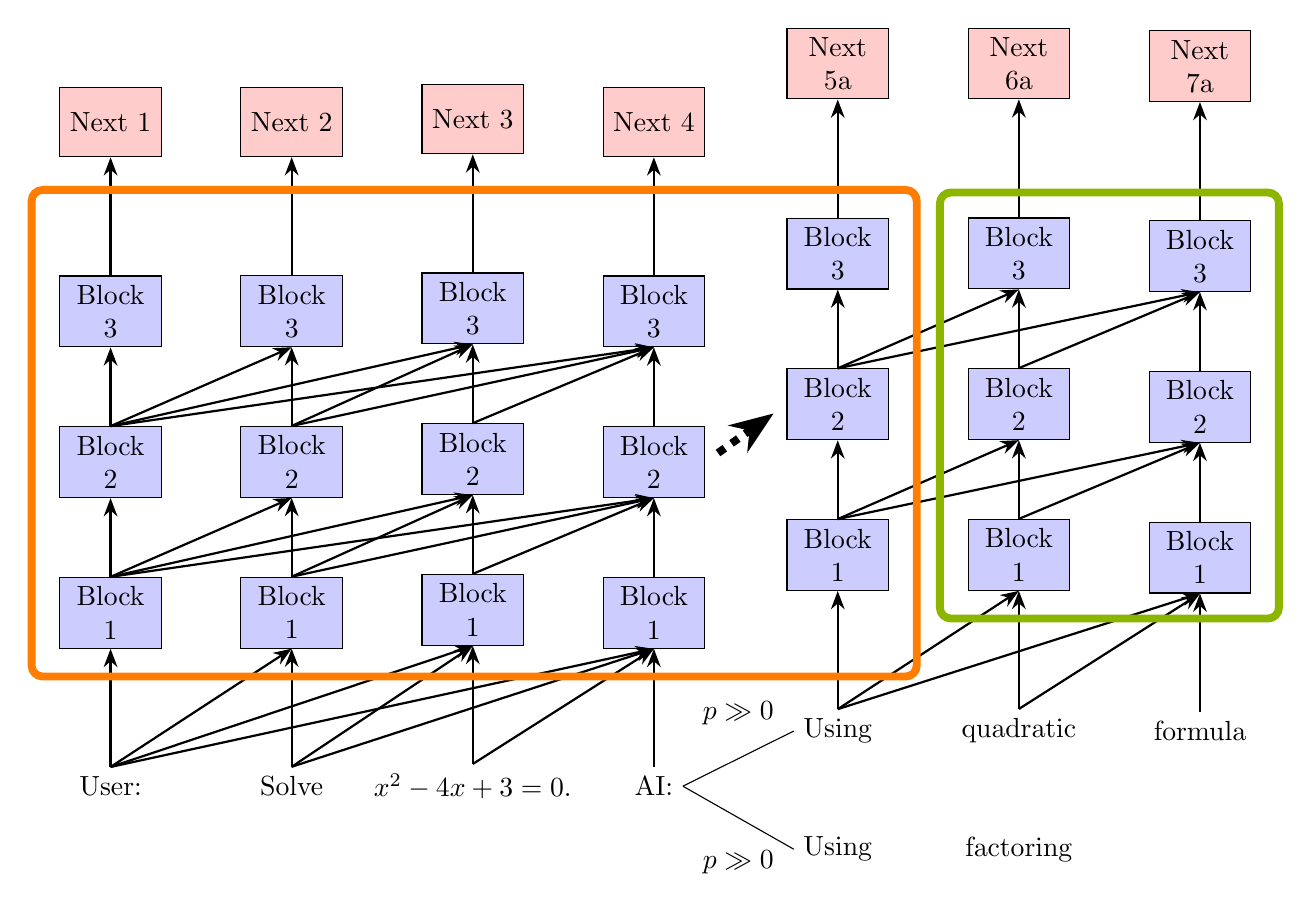
\begin{tikzpicture}[block/.style={rectangle, draw, fill=blue!20, text width=3em, text centered, minimum height=2.5em}, 
                    output/.style={rectangle, draw, fill=red!20, text width=3em, text centered, minimum height=2.5em},
                    arrow/.style={-Stealth, thick}]

  % Definitions for layers, nodes per layer, vertical spacing, and branching nodes
  \def\layers{3}
  \def\nodesPerLayer{4}
  \def\horizontalSpacing{2.3cm}
  \def\verticalSpacingInput{1.5cm}
  \def\verticalSpacing{1cm}
  \def\verticalSpacingOutput{1.5cm}
  \def\branchNodes{3}

  % Generate input nodes
%   \foreach \n in {1,...,\nodesPerLayer} {
%     \node at (\n*2, 0) (input\n) {Word \n};
%   }

  \node at (\horizontalSpacing, 0) (input1) {User:};
  \node at (\horizontalSpacing*2, 0) (input2) {Solve};
  \node at (\horizontalSpacing*3, 0) (input3) {$x^2 - 4x + 3 = 0$.};
  \node at (\horizontalSpacing*4, 0) (input4) {AI:};

  % Branching inputs for top path
%   \foreach \n in {1,...,\branchNodes} {
%     \node at (\horizontalSpacing*\nodesPerLayer + \n*\horizontalSpacing + 1, 0.7cm) (inputA\n) {Word \the\numexpr 3+\n\relax a};
%   }

  \node at (\horizontalSpacing*\nodesPerLayer + 1*\horizontalSpacing + 1, 0.7cm) (inputA1) {Using};
  \node at (\horizontalSpacing*\nodesPerLayer + 2*\horizontalSpacing + 1, 0.7cm) (inputA2) {quadratic};
  \node at (\horizontalSpacing*\nodesPerLayer + 3*\horizontalSpacing + 1, 0.7cm) (inputA3) {formula};

  % Branching inputs for bottom path (text only)
%   \foreach \n in {1,...,2} {
%     \node at (\horizontalSpacing*\nodesPerLayer + \n*\horizontalSpacing + 1, -0.8cm) (inputB\n) {Word \the\numexpr 3+\n\relax b};
%   }

  \node at (\horizontalSpacing*\nodesPerLayer + 1*\horizontalSpacing + 1, -0.8cm) (inputB1) {Using};
  \node at (\horizontalSpacing*\nodesPerLayer + 2*\horizontalSpacing + 1, -0.8cm) (inputB2) {factoring};

  \draw (input\nodesPerLayer.east) -- node[above=3mm] {$p \gg 0$} (inputA1.west);
  \draw (input\nodesPerLayer.east) -- node[below=3mm] {$p \gg 0$} (inputB1.west);

  % Generate transformer blocks and connect them with causal attention for main path
  \foreach \l in {1,...,\layers} {
    \foreach \n in {1,...,\nodesPerLayer} {
      \ifnum\l=1
        \node[block, above=\verticalSpacingInput of input\n] (block\l-\n) {Block \l};
      \else
        \node[block, above=\verticalSpacing of block\the\numexpr\l-1\relax-\n] (block\l-\n) {Block \l};
      \fi

      % Connect nodes from previous layer to current block with causal attention
      \ifnum\l>1
        \foreach \m in {1,...,\n} {
          \draw[arrow] (block\the\numexpr\l-1\relax-\m.north) -- (block\l-\n.south);
        }
      \else % For layer 1, connect input nodes to all subsequent block nodes
        \foreach \m in {1,...,\n} {
          \draw[arrow] (input\m.north) -- (block\l-\n.south);
        }
      \fi
    }
  }

  % Continue transformer blocks and connections for the top path
  \foreach \l in {1,...,\layers} {
    \foreach \n in {1,...,\branchNodes} {
      \ifnum\l=1
        \node[block, above=\verticalSpacingInput of inputA\n] (blockA\l-\n) {Block \l};
      \else
        \node[block, above=\verticalSpacing of blockA\the\numexpr\l-1\relax-\n] (blockA\l-\n) {Block \l};
      \fi

      \ifnum\l>1
        \foreach \m in {1,...,\n} {
          \draw[arrow] (blockA\the\numexpr\l-1\relax-\m.north) -- (blockA\l-\n.south);
        }
      \else % For layer 1 in top path, connect to all subsequent block nodes
        \foreach \m in {1,...,\n} {
          \draw[arrow] (inputA\m.north) -- (blockA\l-\n.south);
        }
      \fi
    }
  }

  \draw[arrow, dashed, line width=1mm, shorten <=2mm, shorten >=2mm] (block2-\nodesPerLayer.east) -- (blockA2-1.west);

  % Generate output nodes for main and top path, and connect them
  \foreach \n in {1,...,\nodesPerLayer} {
    \node[output, above=\verticalSpacingOutput of block\layers-\n] (output\n) {Next \n};
    \draw[arrow] (block\layers-\n.north) -- (output\n.south);
  }

  \foreach \n in {1,...,\branchNodes} {
    \node[output, above=\verticalSpacingOutput of blockA\layers-\n] (outputA\n) {Next \the\numexpr 4+\n\relax a};
    \draw[arrow] (blockA\layers-\n.north) -- (outputA\n.south);
  }

  \definecolor{ao(english)}{rgb}{0.0, 0.5, 0.0}
  \definecolor{applegreen}{rgb}{0.55, 0.71, 0.0}
  \definecolor{amber(sae/ece)}{rgb}{1.0, 0.49, 0.0}
  \node[rectangle, rounded corners=5mm, draw=amber(sae/ece), line width=1mm, inner sep=10pt, fit=(block1-1) (blockA3-1), rounded corners] {};
  \node[rectangle, rounded corners=5mm, draw=applegreen, line width=1mm, inner sep=10pt, fit=(blockA1-2) (blockA3-3), rounded corners] {};
  
\end{tikzpicture}

\end{document}
